\documentclass[12pt]{beamer}

\usepackage[utf8]{inputenc}
\usepackage{amsmath}
\usepackage{hyperref}
\usepackage{graphicx}
\usepackage{caption}
\usepackage{subcaption}
\usepackage[style=ext-authoryear, backend=biber]{biblatex}
\addbibresource{refs.bib}

\DeclareOuterCiteDelims{parencite}{\bibopenbracket}{\bibclosebracket}

\begin{document}
\begin{frame}{MetaRL for Non-stationary and -parametric Environments \parencite{paper}}
  \begin{itemize}
    \item often task changes over time
    \item especially if a task is comprised of subtasks
    \pause
    \item[$\rightarrow$] generate task-embedding via VAE
  \end{itemize}
  \begin{figure}[h]
    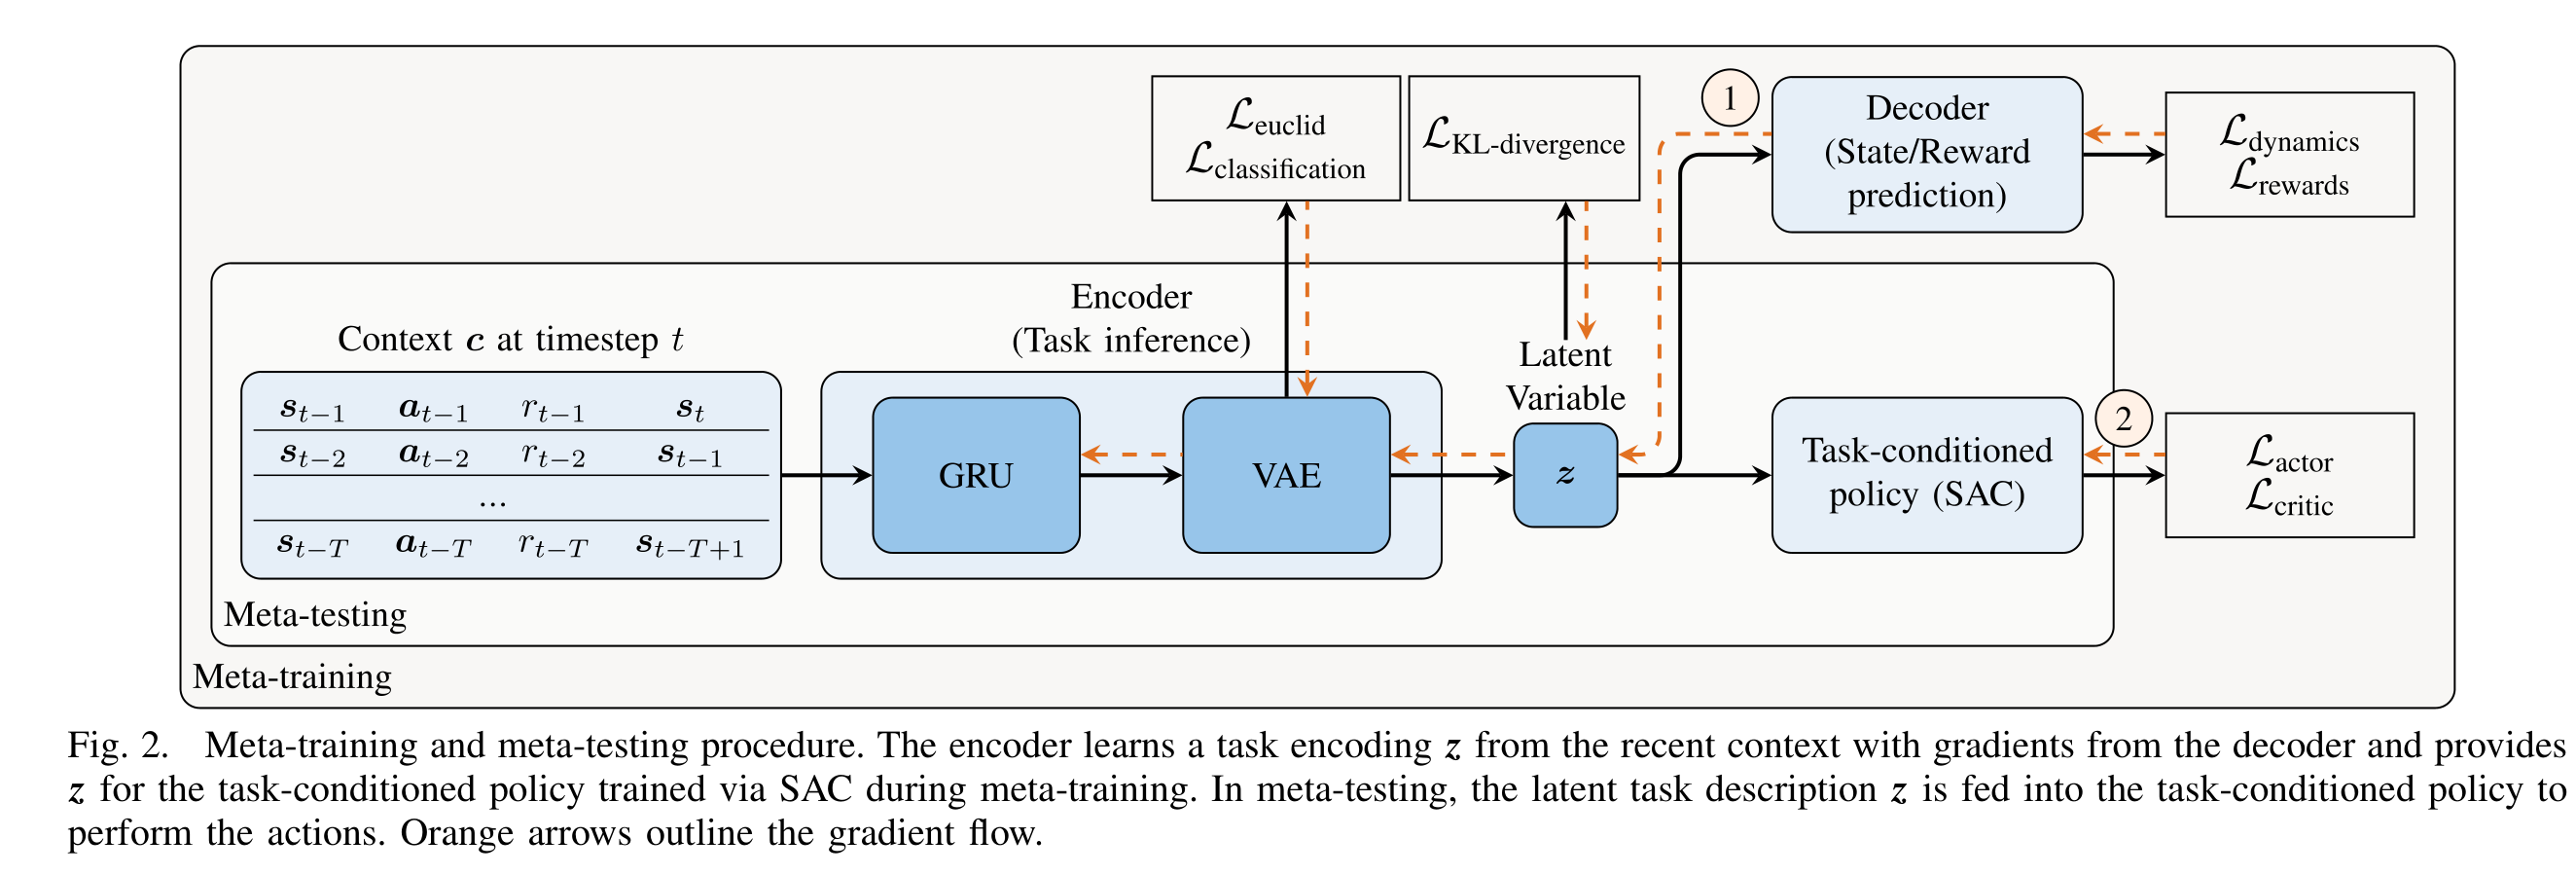
\includegraphics[width=\textwidth]{./diagram.png}
  \end{figure}
\end{frame}

\begin{frame}
  \begin{figure}
    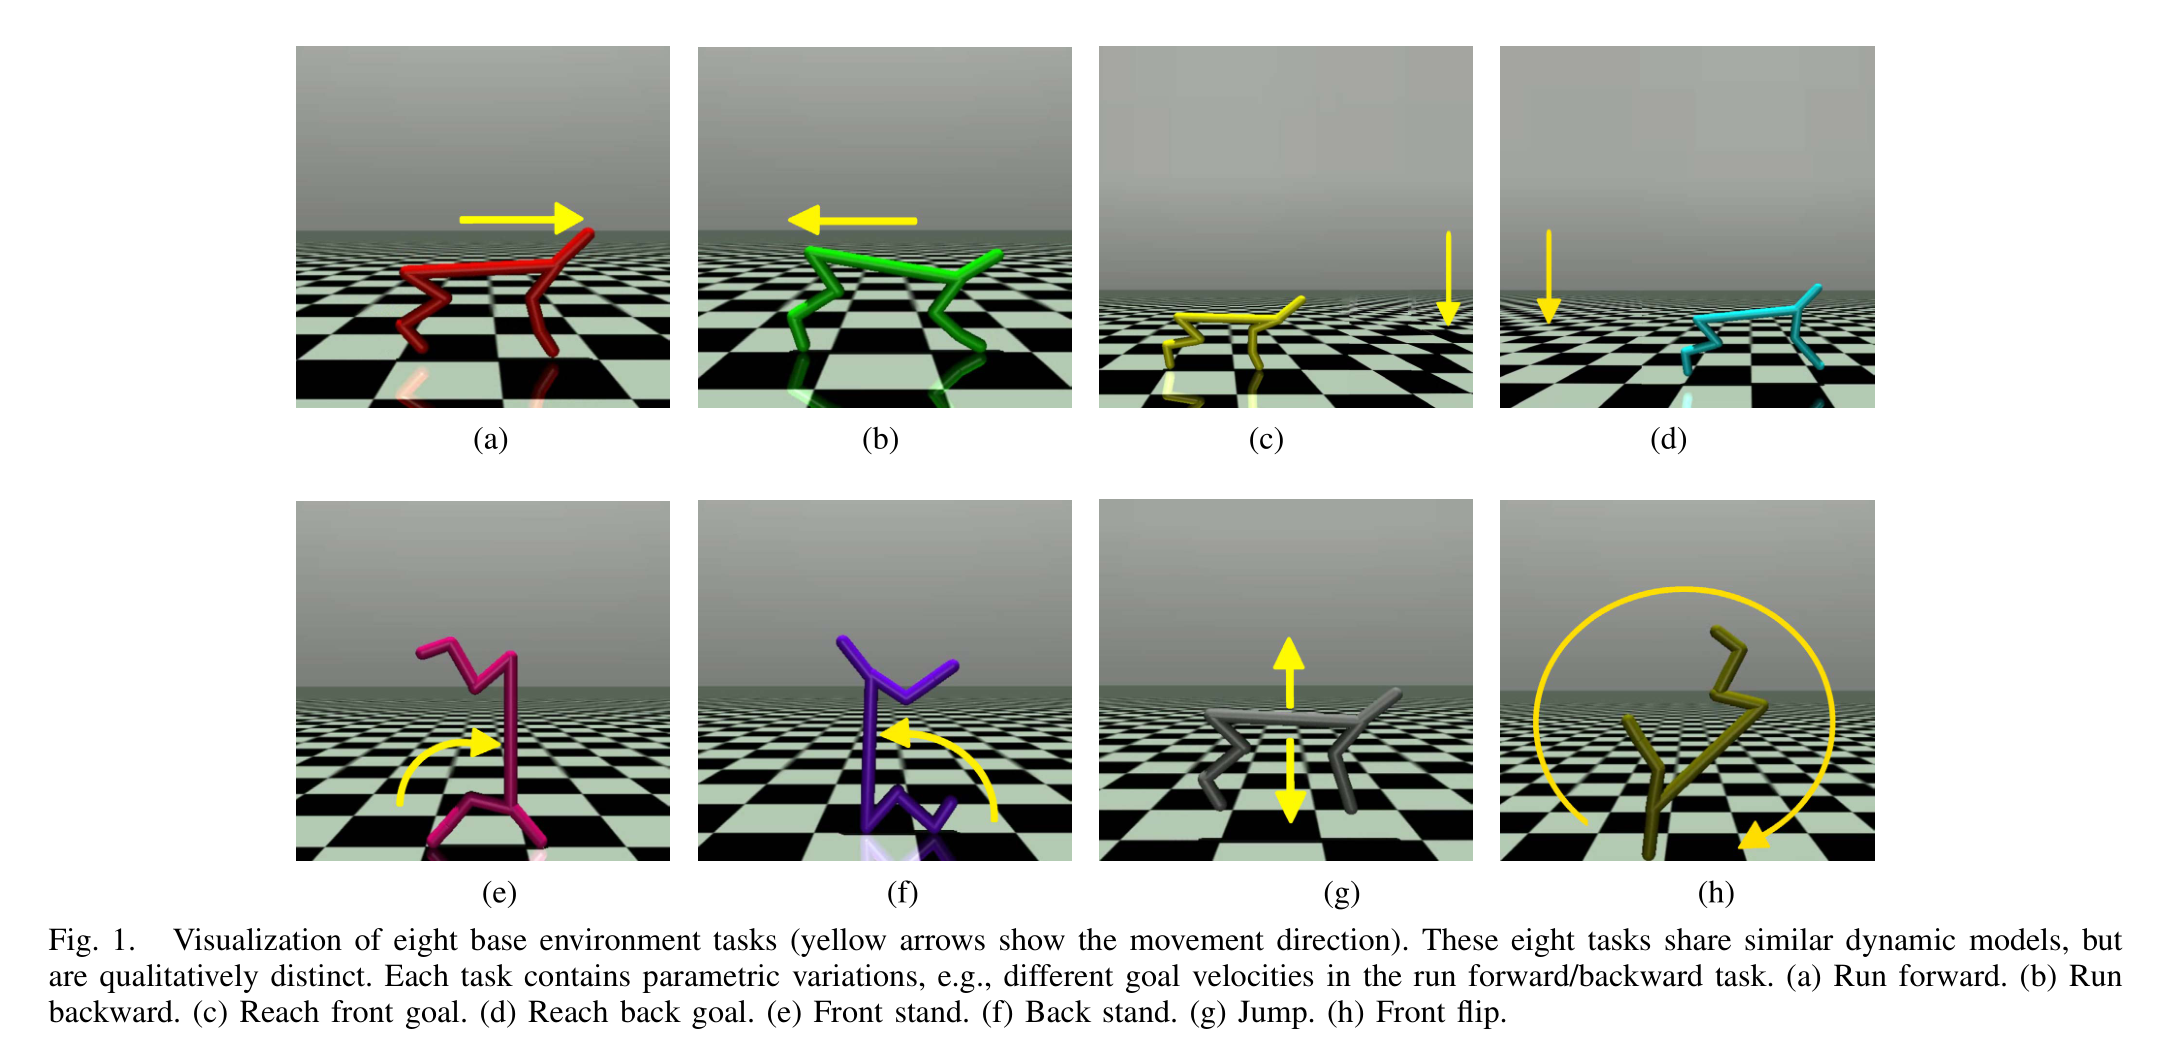
\includegraphics[height=0.5\textheight]{./half-cheetah-eight.png}
  \end{figure}
  \begin{figure}
    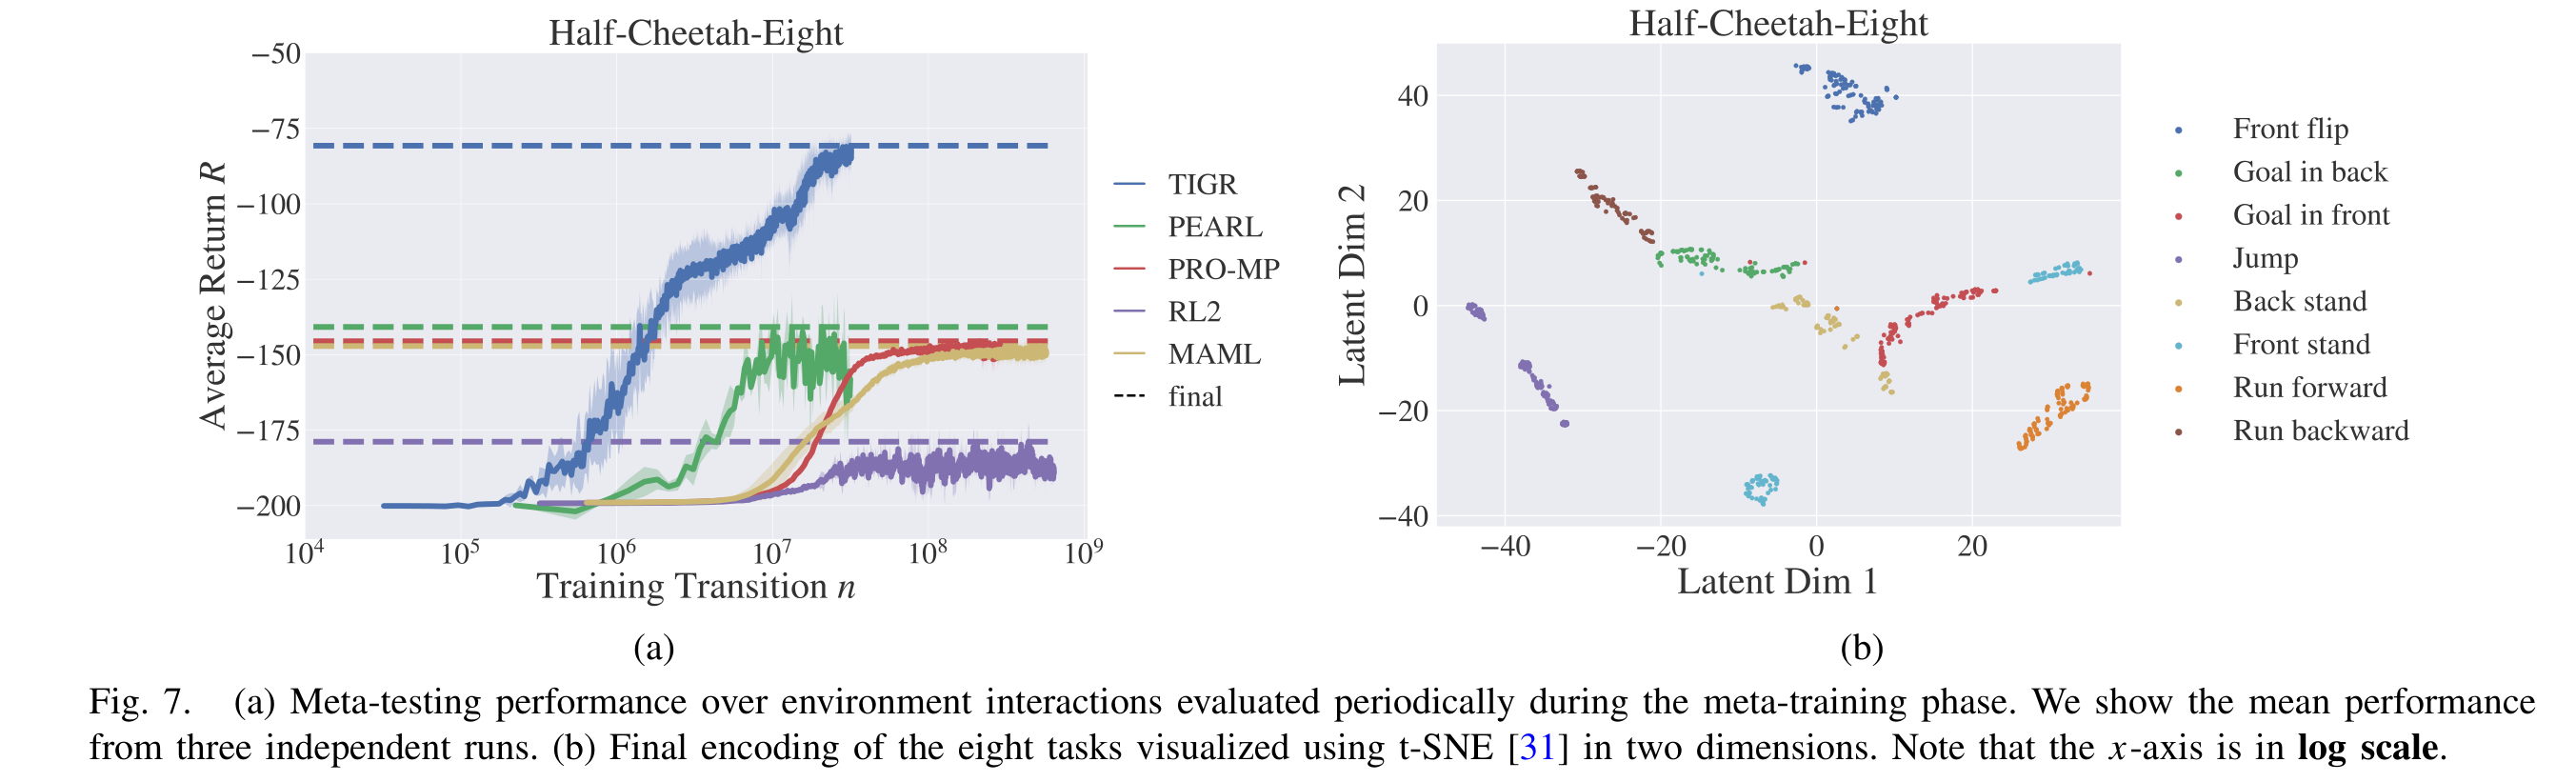
\includegraphics[height=0.5\textheight, width=\textwidth, keepaspectratio]{./evaluation.png}
  \end{figure}
\end{frame}

\end{document}
